	\begin{center}
		\psset{xunit=2.5cm,yunit=1.5cm,labelFontSize=\scriptstyle,showorigin=false,comma=true}
		\begin{pspicture}(-3,-3)(3,2.6)
			\multido{\n=-2.5+0.1}{50}{\psline[linewidth=0.35pt,linecolor=lightgray](\n,-2.9)(\n,2.4)}
			\multido{\n=-2.9+0.1}{54}{\psline[linewidth=0.35pt,linecolor=lightgray](-2.5,\n)(2.4,\n)}
			\multido{\n=-2.5+0.5}{10}{\psline[linewidth=0.45pt](\n,-2.9)(\n,2.4)}
			\multido{\n=-2.5+0.5}{10}{\psline[linewidth=0.45pt](-2.5,\n)(2.4,\n)}
			\psaxes[linewidth=0.95pt,Dx=0.5,Dy=0.5]{->}(0,0)(-2.5,-2.9)(2.5,2.4)
			\def\Func{x x x 1 add mul 1 sub mul 1 sub}
			\psplot[plotpoints=2000,linewidth=1.25pt,linecolor=red]{-1.986}{1.412}{\Func}
			\def\Func{x x x 1 add mul mul}
			\psplot[plotpoints=2000,linewidth=1.25pt,linecolor=green]{-1.849}{1.075}{\Func}
			\def\Func{x 1 add}
			\psplot[plotpoints=2000,linewidth=1.25pt,linecolor=blue]{-2.5}{1.4}{\Func}
			\psline[linewidth=1.25pt](-2.5,-1.185185)(2.4,-1.185185)
			\psdots[dotstyle=Mul,dotscale=2.06,linecolor=blue](-1,0)(0.333333,-1.185185)
			\uput[u](-1,0){$A$}\uput[d](0.333333,-1.185185){$B$}\uput[dl](0,0){O}\uput[r](1.01,1.3){\red $\mathcal{C}_f$} \uput[r](0.45,1.1){\green $\mathcal{C}_g$} \uput[d](2.2,-1.25){$T_B$}
		\end{pspicture}
	\end{center}
	
	1. On lit sur la figure \( f(-1) = 0 \) et \( f(1) = 0 \).
	
	La fonction \( f \) est définie sur \( \mathbb{R} \) par \( f(x) = x^3 + x^2 - x - 1 \). On note \( f' \) la dérivée de \( f \).
	
	2. La fonction polynôme \( f \) est dérivable sur \( \mathbb{R} \) et sur cet intervalle :
	\[
	f'(x) = 3x^2 + 2x - 1.
	\]
	3. On sait que \( f'(x) \) s'annule pour \( x = -1 \) et pour \( x = \dfrac{1}{3} \).
	
	Comme \( f'(x) = 3(x - \alpha)(x - \beta) \), avec \( a \) coefficient de \( x^2 \), \( \alpha \) et \( \beta \) racines du trinôme, on a :
	\[
	f'(x) = 3 \left( x - \dfrac{1}{3} \right) (x - (-1)) = 3 \left( x - \dfrac{1}{3} \right) (x + 1).
	\]
	On sait que ce trinôme est du signe de \( a = 3 \), donc positif sauf dans l'intervalle \( \left] -1 \, ; \, \dfrac{1}{3} \right[ \).
	
\begin{center}
	\begin{tikzpicture}[double distance=2pt]
		\tkzTabInit[lgt=3,espcl=2]{$x$/1,$f'(x)$/1,$f(x)$/2}{$-\infty$,$-1$, $\dfrac{1}{3}$,$+\infty$}
		\tkzTabLine{,+,z,-,z,+}
		\tkzTabVar{-/ , +/0  , -/  , +/}
	\end{tikzpicture}
\end{center}

	
	La fonction \( f \) est donc croissante sauf sur l'intervalle \( \left] -1 \, ; \, \dfrac{1}{3} \right[ \), où elle est décroissante (ce que conforte la figure donnée).
	
	4. Des variations précédentes, on constate que :
	\begin{itemize}
		\item $f(x) < 0$ sur $ ]-\infty \,;\, 1[$ 
		\item $f(x) > 0$  sur $]1 \,;\, +\infty[$.
	\end{itemize}
	
	La fonction \(d\) définie sur \(\mathbb{R}\) par :
	\[
	d(x) = g(x) - (x + 1) = x^3 + x^2 - x - 1 = f(x)
	\]
	donne la différence pour deux points d'abscisse \(x\) entre leurs images par \(g\) et par \(x \mapsto x + 1\).
	
	Or les variations précédentes de \(f\) montrent que :
	\begin{itemize}[label=-]
		\item \(f(x) < 0\) sur \( ]-\infty \,;\, 1[ \) ; autrement dit \(x^3 + x^2 < x + 1\), soit la courbe \(C_g\) est en-dessous de la droite d'équation \(y = x + 1\);
		\item \(f(x) > 0\) sur \( ]1 \,;\, +\infty[ \) ; autrement dit \(x^3 + x^2 > x + 1\), soit la courbe \(C_g\) est au-dessus de la droite d'équation \(y = x + 1\).
	\end{itemize}
	
